\setchapterimage[6cm]{chapter/programming_language/SJ_skyline_at_night_horizontal.jpg}
\setchapterpreamble[u]{\margintoc}
\chapter{Programming languages and its creators\protect\footnotemark}
\labch{programming_language}

\footnotetext{Panorama of San Jose, the unofficial capital of \href{https://en.wikipedia.org/wiki/Silicon_Valley}{Silicon Valley}. Silicon Valley is a region in the southern part of the San Francisco Bay Area in Northern California that serves as a global center for high technology and innovation.
Author: \href{https://commons.wikimedia.org/wiki/File:SJ_skyline_at_night_horizontal.jpg}{Ben Loomis, WikiCommons / 2014 / Creative Commons Attribution License}.}

\section{Abstract}
The chapter examines the properties of programming languages based on the knowledge base of the international project Wikidata. A number of problems have been solved with the help of SPARQL queries calculated on objects of the ``programming language''  type in Wikidata. Lists of all programming languages under permissive licenses and languages with closed licenses were obtained and their percentage was calculated. A bubble chart showing the number of source code file formats was built. Maps have been generated showing the location of educational institutions and companies in which people associated with the creation of programming languages studied or worked. A bubble diagram shows the professions of people involved in the creation and development of programming languages. A list of all object-oriented programming languages was obtained and a conclusion was drawn about the completeness of Wikidata regarding them. Comparison and analysis of the results of SPARQL queries of 2017 and 2020 are carried out, the main changes are noted, such as the filling level of objects, an increase in the number of professions of the creators of programming languages, etc.

\section{List of programming languages}
Objects Used in SPARQL Queries:
\begin{itemize}
	\item\href{https://www.wikidata.org/wiki/Q9143}{programming language}~--- programming language;
	\item\href{https://www.wikidata.org/wiki/Q899523}{object-based language}~--- object-oriented programming language.
\end{itemize}
Properties Used in SPARQL Queries:
\begin{itemize}
	\item\href{https://www.wikidata.org/wiki/Property:P737}{influenced by}~--- which programming languages have influenced;
	\item\href{https://www.wikidata.org/wiki/Property:P178}{developer}~--- who developed the programming language;
	\item\href{https://www.wikidata.org/wiki/Property:P275}{copyright license}~--- what license;
	\item\href{https://www.wikidata.org/wiki/Property:P31}{instance of}~--- what more general type(s) is this language;
	\item\href{https://www.wikidata.org/wiki/Property:P1195}{file extension}~--- file extension;
	\item\href{https://www.wikidata.org/wiki/Property:P159}{headquarters location}~---  location of the headquarters of the language developers;
	\item\href{https://www.wikidata.org/wiki/Property:P625}{coordinate location}~--- \href{https://en.wikipedia.org/wiki/Geographic_coordinate_system}{geographic coordinates} of the object;
	\item\href{https://www.wikidata.org/wiki/Property:P69}{educated at}~--- where the object studied;
	\item\href{https://www.wikidata.org/wiki/Property:P19}{place of birth}~--- where the object was born;
	\item\href{https://www.wikidata.org/wiki/Property:P106}{occupation}~--- object's occupation (profession).
\end{itemize}
We study information about programming languages in Russian Wikipedia, English Wikipedia and Wikidata. Let's build a list of all languages (Listing \ref{lst:prog_languages}).
\begin{lstlisting}[ language=SPARQL, 
                    caption={List of programming languages.\\\hspace{\textwidth}
                        The result contains \num{732} languages in 2017, 
                        \num{1422} languages in 2020.\\\hspace{\textwidth}
                        SPARQL query: \href{https://w.wiki/uG3}{w.wiki/uG3}
                        },
                    label=lst:prog_languages,
                    texcl 
                    ]
#List of `instances of` "programming language" 
SELECT ?lang ?langLabel
WHERE
{
    ?lang wdt:P31 wd:Q9143. # instances of programming language
    SERVICE wikibase:label { bd:serviceParam wikibase:language "en" }
}
\end{lstlisting}%

The most complete and well-developed programming languages on Wikidata for 2017 were: \wdqName{Java}{251}, \wdqName{Python}{28865}, \wdqName{C}{15777}. For 2020 the most well-developed programming languages on Wikidata are: \wdqName{C++}{2407} (26 properties), \wdqName{Java}{251} (26 properties), \wdqName{JavaScript}{2005} (25 properties), \wdqName{R}{206904} (25 properties).

Almost empty and uninformative languages for 2020 are: \wdqName{Proteus}{3924253}, \wdqName{Cryptol}{5190950}, \wdqName{Flow Java}{5462069}, \wdqName{Comfy}{21524853} according to ProWD\cite{prowd_langs}.

In 2017 there were languages with an unfilled label, but script \ref{lst:labled_prog_languages} shows that for 2020 all languages have a filled label. However, not all programming languages have labels for the Russian language.

\begin{lstlisting}[ language=SPARQL, 
                    caption={List of programming languages with label.\\\hspace{\textwidth}
                        The result contains \num{709} languages in 2017, 
                        \num{1422} languages in 2020.\\\hspace{\textwidth}
                        SPARQL query: \href{https://w.wiki/uG7}{w.wiki/uG7}
                        },
                    label=lst:labled_prog_languages,
                    texcl 
                    ]
#List of `instances of` "programming language" only with a label.
SELECT ?lang ?lang_label
WHERE
{
    ?lang wdt:P31 wd:Q9143
    ; rdfs:label ?lang_label FILTER (LANG(?lang_label) = "en") . 
}
\end{lstlisting}%
For 2020, all languages in the list have a filled label field.

\label{question:prog_lang_1}
\marginnote{
Match a programming language and its developer.
\newline
	\begin{tabular}{ll}
		Developer & Language\\
		\hline
		\href{https://en.wikipedia.org/wiki/Jean_Ichbiah}{J.Ichbiah} & \href{https://www.wikidata.org/wiki/Q154755}{Ada}\\
		\href{https://en.wikipedia.org/wiki/Charles_H._Moore}{C.Moore} & \href{https://www.wikidata.org/wiki/Q275472}{Forth}\\
		\href{https://en.wikipedia.org/wiki/Joe_Armstrong_(programmer)}{J.Armstrong} & \href{https://www.wikidata.org/wiki/Q334879}{Erlang}\\
	\end{tabular}
\newline
The answer is on page~\pageref{answer:prog_lang_1}.
}

\section{Demonstration of work with operations on sets in SPARQL}

Let us list all programming languages that are open (free) software and influenced by at least one of the following programming languages: \wdqName{C}{15777}, \wdqName{Python}{28865}, \wdqName{Java}{251} and not developed by any of the companies, except: \href{https://en.wikipedia.org/wiki/Sun_Microsystems}{Sun Microsystems}, \href{https://en.wikipedia.org/wiki/Johnson_Space_Center}{Johnson Space Center} (Listing~\ref{lst:prog_lang_sets}).
\index{SPARQL!MINUS!An example of working with sets.}
\begin{lstlisting}[ language=SPARQL, 
                    caption={List of free programming languages influenced by C, Python or Java and not developed by Sun Microsystems or Johnson Space Center.\\\hspace{\textwidth}
                        The result contains \num{115} languages in 2017, 
                        \num{122} languages in 2020.\\\hspace{\textwidth}
                        SPARQL query: \href{https://w.wiki/kCh}{w.wiki/kCh}
                        },
                    label=lst:prog_lang_sets,
                    texcl 
                    ]
SELECT DISTINCT ?lang ?lang_label
WHERE
{
    ?lang wdt:P31 wd:Q9143
    ; rdfs:label ?lang_label FILTER (LANG(?lang_label) = "en") . 
    {
      { ?lang wdt:P737 wd:Q15777 } UNION
      { ?lang wdt:P737 wd:Q28865 } UNION 
      { ?lang wdt:P737 wd:Q251   } UNION
      { ?lang wdt:P31 wd:Q341    }
    } MINUS { 
      { ?lang wdt:P178 wd:Q14647  } UNION
      { ?lang wdt:P178 wd:Q208371 }
    }   
}
\end{lstlisting}%

\section{Permissive licenses}
We will output all programming languages under permissive licenses (practically do not limit freedom of action of users of software and developers).

\begin{lstlisting}[ language=SPARQL, 
                    caption={List of programming languages under permissive licenses.\\\hspace{\textwidth}
                        The result contains \num{37} languages in 2017, 
                        \num{82} languages in 2020.\\\hspace{\textwidth}
                        SPARQL query: \href{https://w.wiki/rc7}{w.wiki/rc7}
                        },
                    label=lst:prog_lang_permissive,
                    texcl 
                    ]
SELECT DISTINCT ?lang ?lang_label
WHERE
{
	?lang wdt:P31 wd:Q9143
	; rdfs:label ?lang_label FILTER (LANG(?lang_label) = "en") . 
	{ ?lang wdt:P275 wd:Q308915  }  UNION  # license Mozzila Public
	{ ?lang wdt:P275 wd:Q334661  }  UNION  # license MIT
	{ ?lang wdt:P275 wd:Q191307  }  UNION  # license BSD
	{ ?lang wdt:P275 wd:Q6905323 }             # license CC
}
\end{lstlisting}%

There were, for example, \href{https://en.wikipedia.org/wiki/CoffeeScript}{CoffeeScript}, \href{https://en.wikipedia.org/wiki/Go}{Go}, \href{https://en.wikipedia.org/wiki/Haml}{Haml}, in this list of 82 "free"\  languages.

Consider the relationship between permissive and proprietary or closed-licensed languages.

\begin{lstlisting}[ language=SPARQL, 
                    caption={Relationship between permissive and proprietary or closed-licensed languages.\\\hspace{\textwidth}
                        For 2020 the ratio is 25\%.\\\hspace{\textwidth}
                        SPARQL query: \href{shorturl.at/beouL}{shorturl.at/beouL}
                        },
                    label=lst:prog_lang_relationship,
                    texcl 
                    ]
#The script calculates the percentage of programming languages 
# with a free license in relation to languages with a closed license
SELECT (COUNT(?not_free)* 100 / (COUNT(?free)) as ?total) WHERE
{{
    SELECT ?free WHERE {
         ?free wdt:P31 wd:Q9143 # instance of prog. language
         ; rdfs:label ?item_label FILTER (LANG(?item_label) = "en") . 
         { ?free wdt:P275 wd:Q308915  }  UNION  # license Mozzila Public
         { ?free wdt:P275 wd:Q334661  }  UNION  # license MIT
         { ?free wdt:P275 wd:Q191307  }  UNION  # license BSD
         { ?free wdt:P275 wd:Q6905323 }         # license CC
    }} UNION {
    SELECT ?not_free WHERE {
      ?not_free wdt:P31 wd:Q9143 # instances of programming language
      ; rdfs:label ?lang_label FILTER (LANG(?lang_label) = "en") .
      { ?not_free wdt:P275 wd:Q6165015 } UNION # Java Research
      { ?not_free wdt:P275 wd:Q218616 } UNION # propr. software
      { ?not_free wdt:P275 wd:Q3238057 } UNION # propr. license 
      { ?not_free wdt:P275 wd:Q31202214 } UNION # propr. software 
      { ?not_free wdt:P275 wd:Q979794 } # Aladdin Free Public
    }
}}
\end{lstlisting}%

\section{Number of source file formats}

Depending on the programming language, the source code files for programs may have different extensions. Let's construct a bubble diagram by the number of valid formats of the source code files.
\index{Chart!BubbleChart!Number of file formats for programming languages}
\begin{lstlisting}[ language=SPARQL, 
                    caption={Number of file formats for programming languages.\\\hspace{\textwidth}
                        SPARQL query: \href{https://w.wiki/kf7}{w.wiki/kf7}
                        },
                    label=lst:prog_lang_file_formats,
                    texcl 
                    ]
#defaultView:BubbleChart
SELECT ?lang_name (count(*) as ?count)
WHERE
{
	?lang wdt:P31 wd:Q9143. # instance of programming language
	?lang wdt:P1195 ?count. # file extension
	?lang rdfs:label ?lang_name FILTER (lang(?lang_name) = "en").
}
GROUP BY ?lang_name 
ORDER BY DESC(?count)
\end{lstlisting}%

\begin{marginfigure}[-15cm]
	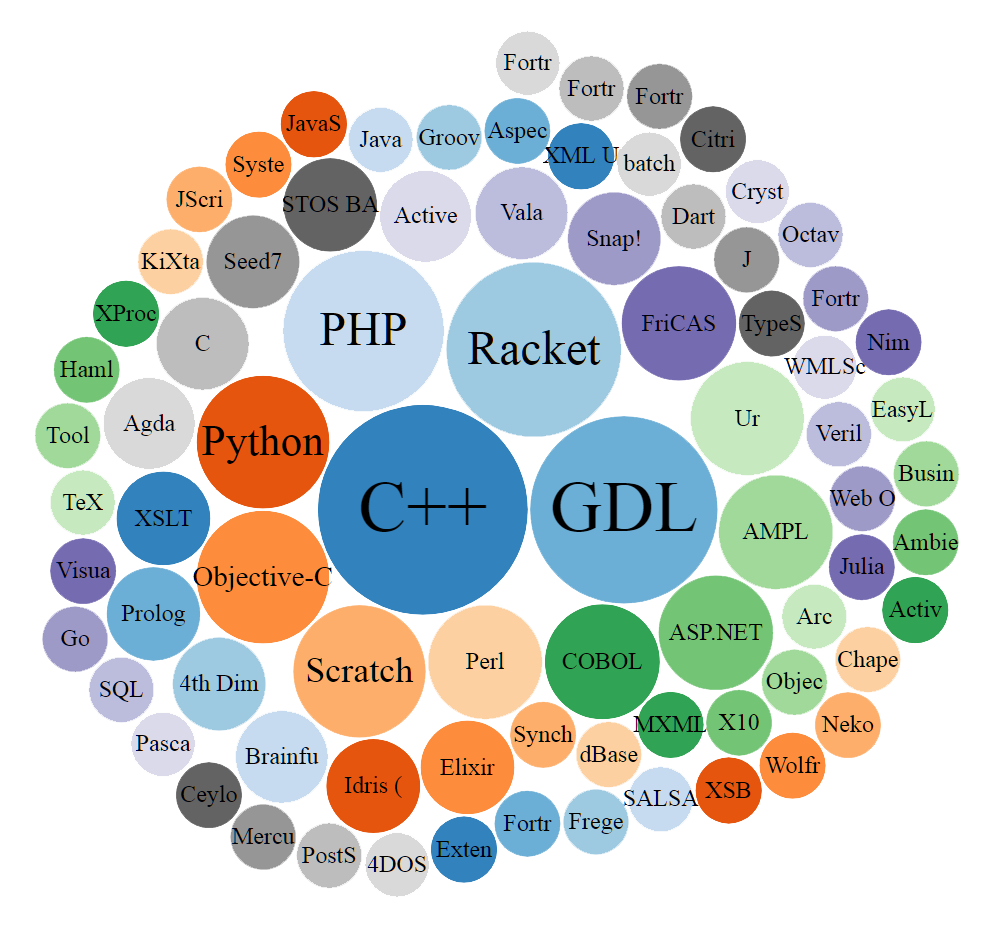
\includegraphics[width=\linewidth]{./chapter/programming_language/File_extensions_quantity_of_source_code_2017.png}
	\caption{Bubble chart by the number of formats of source code files (2017). The size of a bubble of the appropriate format for one language.}
	\label{fig:source_types_2017}
\end{marginfigure}
\begin{marginfigure}[-3cm]
	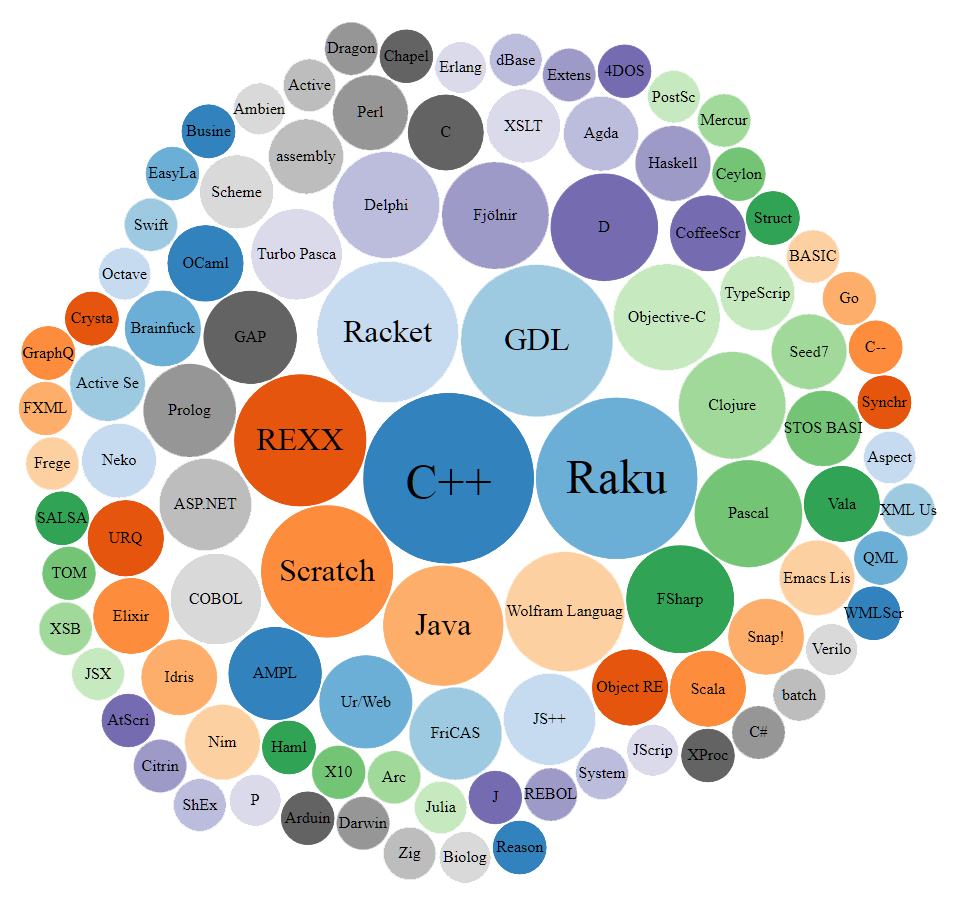
\includegraphics[width=\linewidth]{./chapter/programming_language/File_extensions_quantity_of_source_code_2020.png}
	\caption{Bubble chart by the number of formats of source code files (2020). The size of a bubble of the appropriate format for one language.}
	\label{fig:source_types_2020}
\end{marginfigure}

The figure~\ref{fig:source_types_2017} shows that the most historically rich in formats and file extensions programming languages are \href{https://en.wikipedia.org/wiki/C\%2B\%2B}{C++} (10 formats), \href{https://en.wikipedia.org/wiki/Geometric_Description_Language}{Geometric Description Language} (8), \href{https://en.wikipedia.org/wiki/Racket}{Racket} (7). For example, files with a program in the Racket language can have the extensions rkt, rktl, rktd, scrbl, plt, ss or scm.

By 2020 (fig.~\ref{fig:source_types_2020}), languages such as  \href{https://en.wikipedia.org/wiki/REXX}{REXX} (6 formats), \href{https://en.wikipedia.org/wiki/Java_(programming_language)}{Java} (5 formats), \href{https://en.wikipedia.org/wiki/Wolfram_Language}{Wolfram Language} (5 formats), \href{https://en.wikipedia.org/wiki/Raku_(programming_language)}{Raku} (9 formats), \href{https://en.wikipedia.org/wiki/Geometric_Description_Language}{GDL} (8 formats) have also started to take the lead.

\section{Where located people and organizations associated with the creation of programming languages}

Let's map (figures~\ref{fig:organizations_2017} \& ~\ref{fig:organizations_2020}) the countries in which people and organizations, connected with the creation of programming languages, live. Noticing that the developer of the language can act both as an organization and as individuals. To determine the location (property: coordinate location) of the organization, we will use the coordinates of its headquarters (property: headquarters location), for the person - the coordinates of the place of his birth (property: place of birth).

\index{Chart!Map!Map of the countries where people and organizations connected with the creation of programming languages live}
\begin{lstlisting}[ language=SPARQL, 
                    caption={Map of the countries where people and organizations connected with the creation of programming languages live.\\\hspace{\textwidth}
                        SPARQL query: \href{https://w.wiki/rcA}{w.wiki/rcA}
                        },
                    label=lst:prog_langs_live,
                    texcl 
                    ]
#defaultView:Map
SELECT ?lang_label ?developer_label ?location_label ?coord
WHERE
{
	 ?lang wdt:P31 wd:Q9143 # instances of programming language
	 ; rdfs:label ?lang_label FILTER (LANG(?lang_label) = "en"). 
	 ?lang wdt:P178 ?developer. # developer
	 ?developer rdfs:label ?developer_label
	FILTER (LANG(?developer_label) = "en"). 
	{ ?developer wdt:P159 ?location. } UNION # headquarters location
	{ ?developer wdt:P19 ?location } # place of birth
	?location rdfs:label ?location_label 
	FILTER (LANG(?location_label) = "en").
 	?location wdt:P625 ?coord. # coordinate location
 	SERVICE wikibase:label { bd:serviceParam wikibase:language "en" } 	
}
\end{lstlisting}%

\label{question:prog_lang_2}
\marginnote[-70pt]{
The images below are the logos of various programming languages. Which logo belongs to the \href{https://www.wikidata.org/wiki/Q513238}{LOLCODE}  programming language?\\
	\begin{tabular}{c}
		
\includegraphics[width=1cm]{./chapter/programming_language/task_2_logo_1.PNG}\\
		
\includegraphics[width=1cm]{./chapter/programming_language/task_2_logo_2.PNG}\\
		
\includegraphics[width=1cm]{./chapter/programming_language/task_2_logo_3.PNG}\\
		
\includegraphics[width=1cm]{./chapter/programming_language/task_2_logo_4.PNG}\\
	\end{tabular}
\newline
The answer is on page~\pageref{answer:prog_lang_2}.
}

\begin{figure}[h]
\centering
	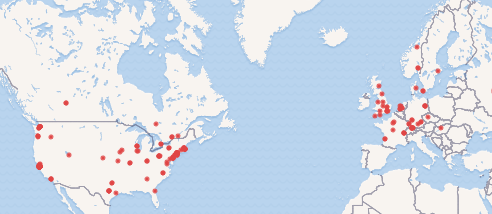
\includegraphics[width=1\textwidth]{./chapter/programming_language/Organizations_map_2017.png}
	\caption{Countries in which people and organizations live, associated with the creation of programming languages (2017).}
	\label{fig:organizations_2017}
\end{figure}

\begin{figure}[h]
\centering
	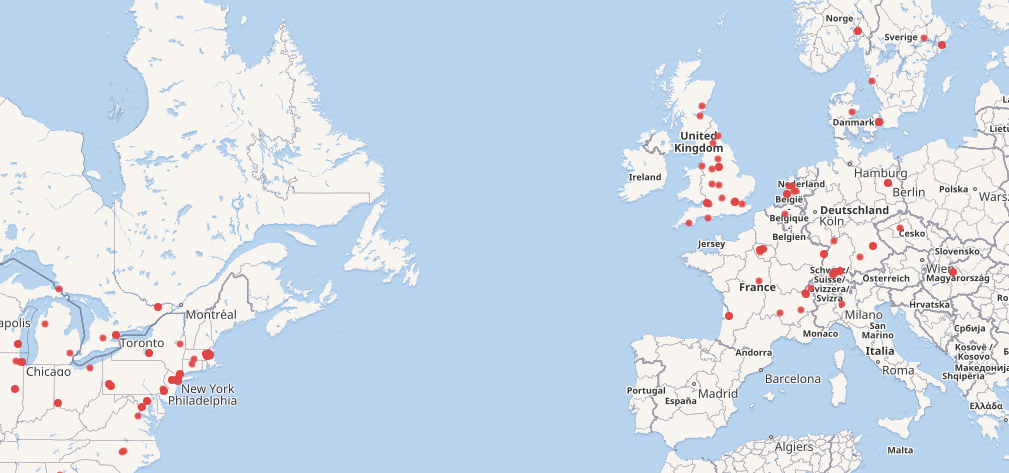
\includegraphics[width=1\textwidth]{./chapter/programming_language/Organizations_map_2020.png}
	\caption{Countries in which people and organizations live, associated with the creation of programming languages (2020)}
	\label{fig:organizations_2020}
\end{figure}

We will also construct a bubble chart (fig.~\ref{fig:emergence_2020}) to identify the most favorable countries for the emergence of people capable of developing programming languages and locating headquarters in these countries. We see in the figure that the most favorable countries were the \href{https://en.wikipedia.org/wiki/United_States}{United States} (159 people and the headquarters of the apartments) and the \href{https://en.wikipedia.org/wiki/United_Kingdom}{United Kingdom} (15). In \href{https://en.wikipedia.org/wiki/Russia}{Russia}, only two programming languages were developed: Refal and the Embedded Programming Language 1C: Enterprise.

\begin{marginfigure}[7cm]
	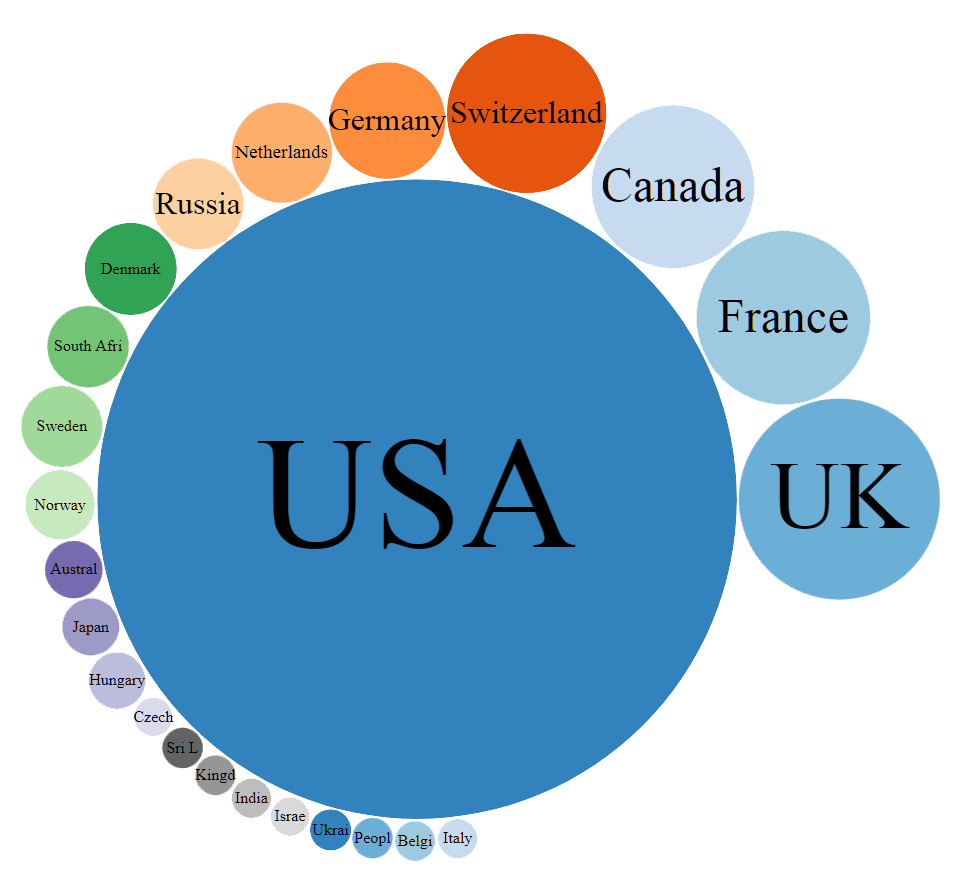
\includegraphics[width=\linewidth]{./chapter/programming_language/The_most_favorable_countries_for_the_emergence_of_people_capable_of_developing_programming_languages_2020.png}
	\caption{Bubble chart of the most favorable countries for the emergence people capable of developing programming languages (2020). The bubble size corresponds to the number of people from the respective country.}
	\label{fig:emergence_2020}
\end{marginfigure}

\index{Chart!BubbleChart!Bubble chart of the most favorable countries for the emergence of people capable of developing programming languages and locating headquarters in these countries}
\begin{lstlisting}[ language=SPARQL, 
                    caption={Bubble chart of the most favorable countries for the emergence of people capable of developing programming languages and locating headquarters in these countries.\\\hspace{\textwidth}
			For 2020, the number of headquarters in the US is 241, in the UK - 24, in France - 18, and in Russia - 5.\\\hspace{\textwidth}
                        SPARQL query: \href{https://w.wiki/n9Q}{w.wiki/n9Q}
                        },
                    label=lst:prog_langs_emerge,
                    texcl 
                    ]
#defaultView:BubbleChart
SELECT ?state_label (count(*) as ?count)
WHERE
{
	?item wdt:P31 wd:Q9143 # instances of programming language
	; rdfs:label ?item_label FILTER (LANG(?item_label) = "en"). 
	?item wdt:P178 ?developer. # developer
	?developer rdfs:label ?developer_label FILTER (LANG(?developer_label) = "en"). 
	{ ?developer wdt:P159 ?location. } UNION # headquarters location
	{ ?developer wdt:P19 ?location } # place of birth
	?location rdfs:label ?location_label FILTER (LANG(?location_label) = "en").
	?location wdt:P17 ?state.
	?state rdfs:label ?state_label FILTER (LANG(?state_label) = "en").
	SERVICE wikibase:label { bd:serviceParam wikibase:language "en" } 	
}
GROUP BY ?state_label
ORDER BY DESC(?count)
\end{lstlisting}%


\section{Universities where people who developed programming languages studied}
Let's display on the map educational institutions, in which students, who subsequently developed programming languages, studied (figures~\ref{fig:institutes_2017} \&~\ref{fig:institutes_2020}).
\index{Chart!Map!Map of educational institutions where developers of programming languages studied}
\begin{lstlisting}[ language=SPARQL, 
                    caption={Map of educational institutions where developers of programming languages studied.\\\hspace{\textwidth}
			The map shows that most of the people involved in the creation of programming languages studied in Europe or the United States.\\\hspace{\textwidth}
                        SPARQL query: \href{https://w.wiki/kDY}{w.wiki/kDY}
                        },
                    label=lst:prog_langs_universities,
                    texcl 
                    ]
#defaultView:Map
SELECT ?item_label ?developer_label ?educational_institution_label ?coord
WHERE
{
	?item wdt:P31 wd:Q9143 # instances of programming language
	; rdfs:label ?item_label FILTER (LANG(?item_label) = "en"). 
	?item wdt:P178 ?developer. # developer
	?developer rdfs:label ?developer_label
	FILTER (LANG(?developer_label) = "en"). 
	?developer wdt:P69 ?educational_institution. # educated at
	?educational_institution rdfs:label ?educational_institution_label
	FILTER (LANG(?educational_institution_label) = "en").
	?educational_institution wdt:P625 ?coord. # coordinate location
	SERVICE wikibase:label { bd:serviceParam wikibase:language "en" } 	
}
\end{lstlisting}%

\label{question:prog_lang_3}
\marginnote{
Fill the gaps.\newline
\href{https://www.wikidata.org/wiki/Q83303}{Fortran} ranks first in terms of the number of its dialects. Their number reaches about \underline{\hspace{1cm}}. In second place is \href{https://www.wikidata.org/wiki/Q132874}{Lisp}, it has \underline{\hspace{1cm}} dialects. The third place is shared by\href{https://www.wikidata.org/wiki/Q597330}{Standard ML} and \href{https://www.wikidata.org/wiki/Q633894}{Object Pascal} with \underline{\hspace{1cm}} dialects.\newline
The answer is on page~\pageref{answer:prog_lang_3}.
}

\begin{figure}[h]
\centering
	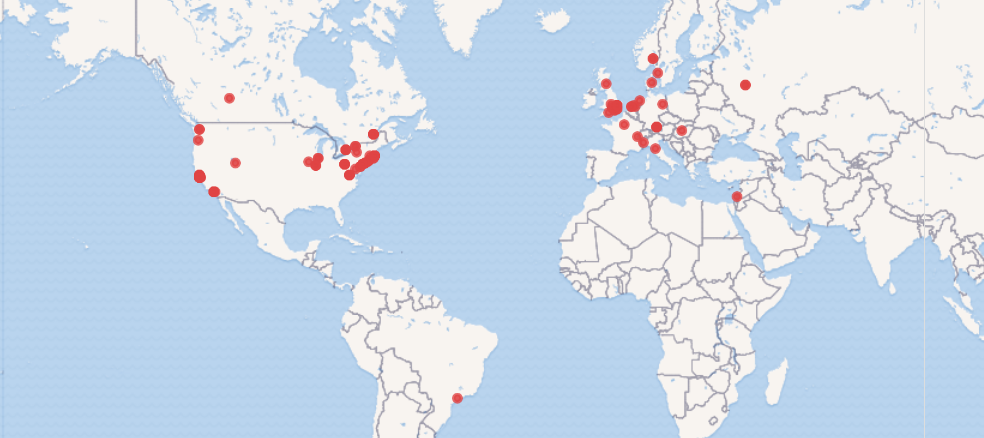
\includegraphics[width=1\textwidth]{./chapter/programming_language/Institutes_2017.png}
	\caption{Educational institutions where developers of programming languages studied. (2017).}
	\label{fig:institutes_2017}
\end{figure}

\begin{figure}[h]
\centering
	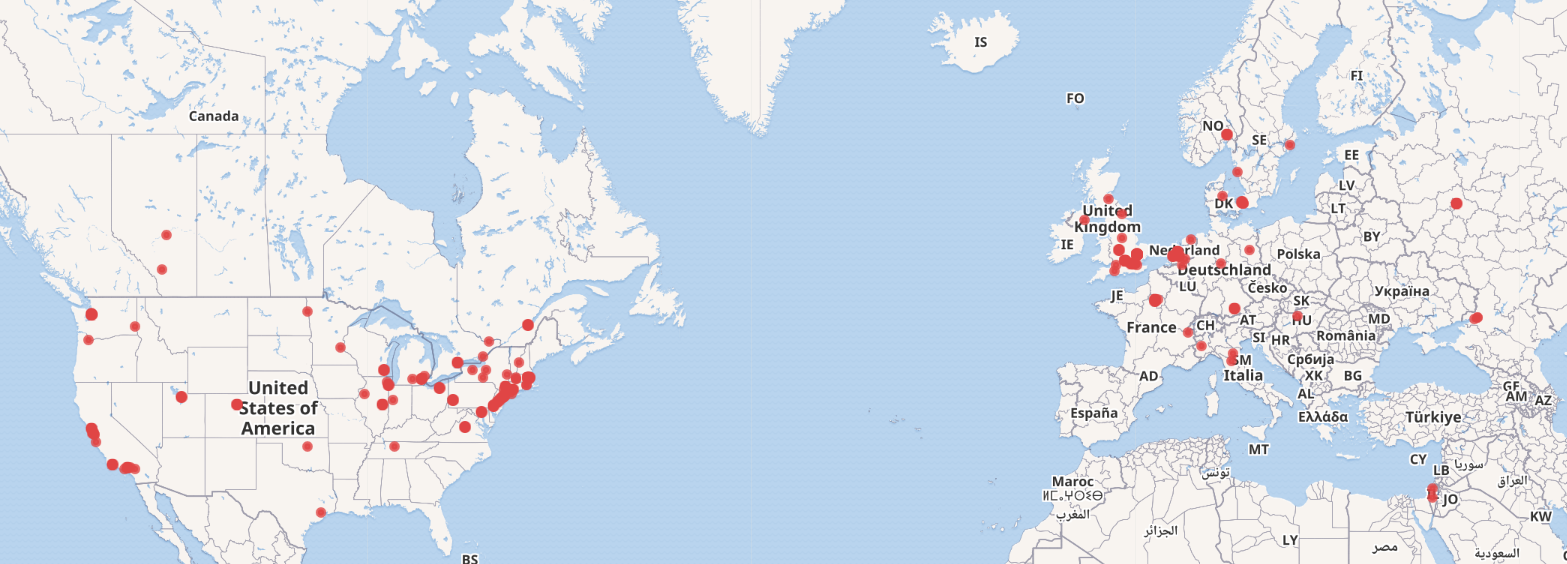
\includegraphics[width=1\textwidth]{./chapter/programming_language/Institutes_2020.png}
	\caption{Educational institutions where developers of programming languages studied. (2020).}
	\label{fig:institutes_2020}
\end{figure}

Let's construct a bubble chart for the most popular educational institutions, among future developers of programming languages (fig.~\ref{fig:universities_2020}). 

\index{Chart!BubbleChart!Bubble chart of the most popular educational institutions, among future developers of programming languages}
\begin{lstlisting}[ language=SPARQL, 
                    caption={Bubble chart of the most popular educational institutions, among future developers of programming languages.\\\hspace{\textwidth}
                        SPARQL query: \href{https://w.wiki/kDb}{w.wiki/kDb}
                        },
                    label=lst:prog_langs_universities_2,
                    texcl 
                    ]
#defaultView:BubbleChart
SELECT ?educational_institution_label (count(*) as ?count)
WHERE
{
	?item wdt:P31 wd:Q9143 # instances of programming language
	; rdfs:label ?item_label FILTER (LANG(?item_label) = "en"). 
	?item wdt:P178 ?developer. # developer
	?developer rdfs:label ?developer_label
	FILTER (LANG(?developer_label) = "en"). 
	?developer wdt:P69 ?educational_institution. # educated at
	?educational_institution rdfs:label ?educational_institution_label
	FILTER (LANG(?educational_institution_label) = "en").
	?educational_institution wdt:P625 ?coord. # coordinate location 
	SERVICE wikibase:label { bd:serviceParam wikibase:language "en" } 	
}
GROUP BY ?educational_institution_label
ORDER BY DESC(?count)
\end{lstlisting}%

\begin{marginfigure}[-7cm]
	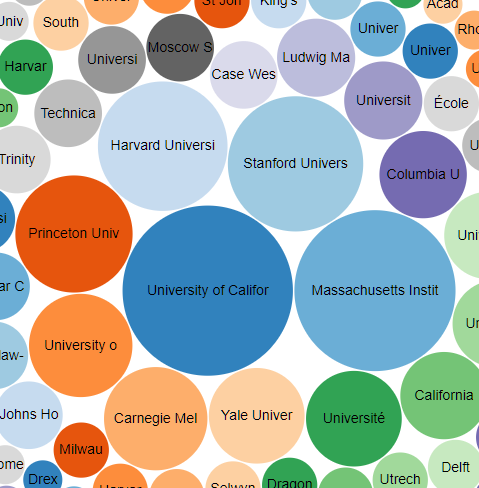
\includegraphics[width=\linewidth]{./chapter/programming_language/Universities_2020.png}
	\caption{Bubble chart of the most favorable universities among future developers of programming languages (2020).}
	\label{fig:universities_2020}
\end{marginfigure}

You can see in the figure~\ref{fig:universities_2020} that the first places were: Berkeley (19), Massachusetts Institute of Technology (17), \href{https://en.wikipedia.org/wiki/Princeton_University}{Princeton University} (9) and \href{https://en.wikipedia.org/wiki/Stanford_University}{Stanford University} (12). MSU was at the end of the list, \href{https://en.wikipedia.org/wiki/Tony_Hoare}{Tony Hoare}, who developed \href{https://en.wikipedia.org/wiki/ALGOL}{ALGOL60}, and \href{https://en.wikipedia.org/wiki/Valentin_Turchin}{Valentin Turchin}, who developed Refal, studied there. Moscow State University was included in this list, which includes 142 universities of the world.

\section{Professions of the creators of programming languages}

\begin{marginfigure}[-5cm]
	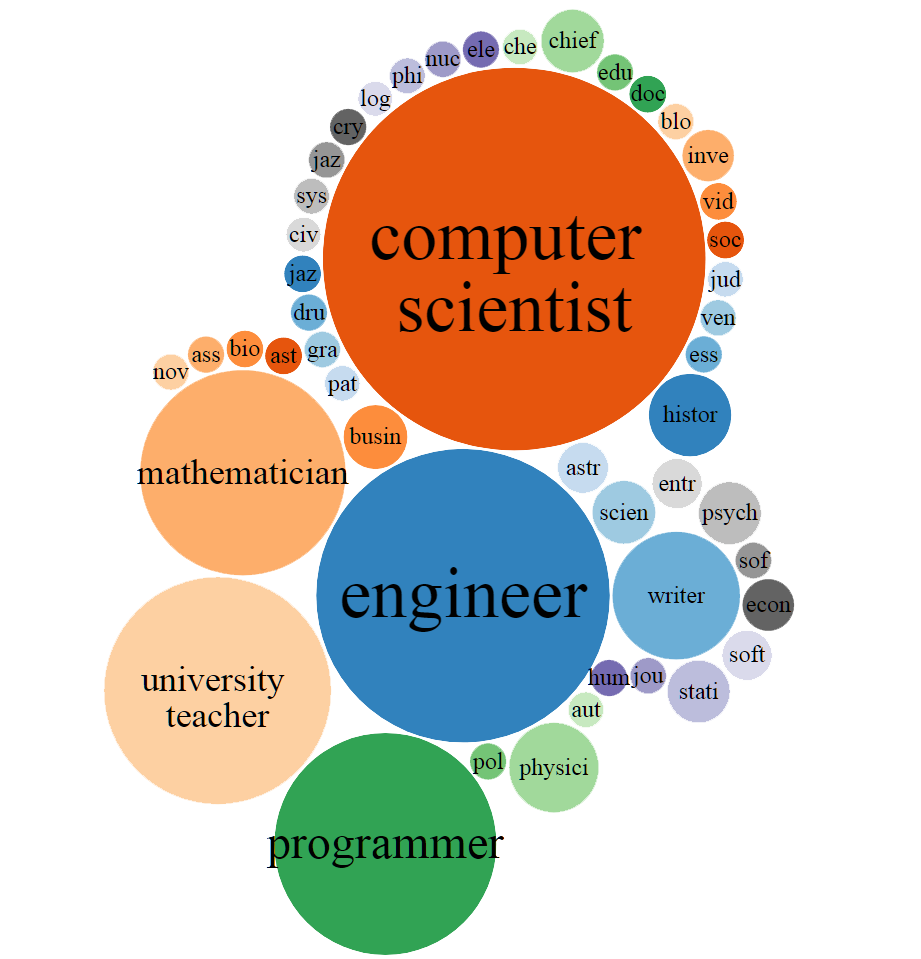
\includegraphics[width=\linewidth]{./chapter/programming_language/Professions_2017.png}
	\caption{Which professions prevail among people developing programming languages (2017).}
	\label{fig:Professions_2017}
\end{marginfigure}

Let's construct a bubble diagram showing which professions prevail among people who develop programming languages.

\index{Chart!BubbleChart!Bubble diagram showing which professions prevail among people who develop programming languages}
\begin{lstlisting}[ language=SPARQL, 
                    caption={Bubble diagram showing which professions prevail among people who develop programming languages.\\\hspace{\textwidth}
			The result contains \num{48} occupations in 2017, 
                        \num{74} occupations in 2020.\\\hspace{\textwidth}
                        SPARQL query: \href{https://w.wiki/kDc}{w.wiki/kDc}
                        },
                    label=lst:prog_langs_occupation,
                    texcl 
                    ]
#defaultView:BubbleChart
SELECT ?occupation_label (count(*) as ?occupation)
WHERE
{
    ?item wdt:P31 wd:Q9143. # instances of programming language 
    ?item wdt:P178 ?developer. # developer
    ?developer wdt:P106 ?occupation. # occupation
    ?occupation rdfs:label ?occupation_label. 
    FILTER (LANG(?occupation_label) = "en"). 
}
GROUP BY ?occupation_label 
ORDER BY DESC(?count)
\end{lstlisting}%

\begin{marginfigure}
	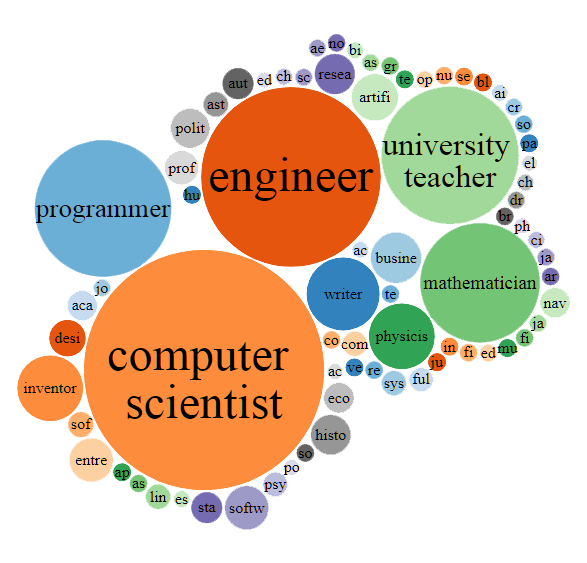
\includegraphics[width=\linewidth]{./chapter/programming_language/Professions_2020.png}
	\caption{Which professions prevail among people developing programming languages (2020).}
	\label{fig:Professions_2020}
\end{marginfigure}

The most common professions (fig.~\ref{fig:Professions_2017}) were: a specialist in computer science, an engineer, a teacher. It is interesting to note that there are such professions as: jazz musician, politician (Herbert A. Simon). In 2020 (fig.~\ref{fig:Professions_2020}), among the developers of programming languages, there were the most specialists in the field of computer science (172 people), as well as 96 engineers, 57 teachers, 56 programmers and 43 mathematicians.

\section{Object-oriented programming languages}

List all object-oriented programming languages.

\begin{lstlisting}[ language=SPARQL, 
                    caption={Object-oriented programming languages.\\\hspace{\textwidth}
			The result contains \num{116} languages in 2017, 
                        \num{118} languages in 2020. Thus, 16\% of programming languages are object-oriented.\\\hspace{\textwidth}
                        SPARQL query: \href{https://w.wiki/kDe}{w.wiki/kDe}
                        },
                    label=lst:prog_langs_oopl,
                    texcl 
                    ]
SELECT DISTINCT ?item ?item_label
WHERE
{
    ?item wdt:P31 wd:Q899523 # instances of object-oriented prog. language
    ; rdfs:label ?item_label FILTER (LANG(?item_label) = "en") 
}
\end{lstlisting}%

\section{Fullness of Wikidata}

According to the Bourabai Research University \cite{oo_langs_bourabai}, there are at least 26 programming languages that support an object-oriented paradigm. In the articles devoted to object-oriented programming, another 4 \cite{oo_langs_science_wikia} and 3 \cite{oo_langs_garshin} programming languages are added to this list. The SPARQL-query (\href{https://w.wiki/n9Y}{w.wiki/n9Y}) returned 116 results. It is difficult to judge the completeness of the data in the three sources cited above, since there are a large number of little-known, obsolete and narrowly focused languages that are not covered in authoritative sources. From this it can be concluded that Wikidata provides a fairly complete list of object-oriented programming languages.

\section{Filling objects}

Let's list all people who are involved in the development of programming languages and whose objects are filled with the 'label' field in English:

\begin{lstlisting}[ language=SPARQL, 
                    caption={List of involved in the development of programming languages with filled with the 'label' field in English.\\\hspace{\textwidth}
			The result contains \num{133} languages in 2017, 
                        \num{223} languages in 2020. \\\hspace{\textwidth}
                        SPARQL query: \href{https://w.wiki/kDg}{w.wiki/kDg}
                        },
                    label=lst:prog_langs_filling_1,
                    texcl 
                    ]
SELECT ?item_label ?item ?developer_label ?developer
WHERE
{
    ?item wdt:P31 wd:Q9143 # instances of programming language
    ; rdfs:label ?item_label FILTER (LANG(?item_label) = "en"). 
    ?item wdt:P178 ?developer. # developer 
    ?developer wdt:P31 wd:Q5.  # instances of human
    ?developer rdfs:label ?developer_label FILTER (LANG(?developer_label) = "en").  
}
\end{lstlisting}%

We will derive a similar list, but with a filled-in 'label' field in Russian. There are 140 such results. Filling in the fields label and description in Russian for these objects and printing the result:

\begin{lstlisting}[ language=SPARQL, 
                    caption={List of involved in the development of programming languages with filled with the 'label' field in Russian.\\\hspace{\textwidth}
			The result contains \num{133} languages in 2017, 
                        \num{183} languages in 2020. \\\hspace{\textwidth}
                        SPARQL query: \href{https://w.wiki/kDj}{w.wiki/kDj}
                        },
                    label=lst:prog_langs_filling_2,
                    texcl 
                    ]
SELECT ?item_label ?item ?developer_label ?developer
WHERE
{
    ?item wdt:P31 wd:Q9143 # instances of programming language
    ; rdfs:label ?item_label FILTER (LANG(?item_label) = "en"). 
    ?item wdt:P178 ?developer. # developer 
    ?developer wdt:P31 wd:Q5.  # instances of human
    ?developer rdfs:label ?developer_label FILTER (LANG(?developer_label) = "en").  
}
\end{lstlisting}%

\section{Exersises}
\begin{enumerate}
\item Output all programming languages with the "\href{https://www.wikidata.org/wiki/Property:P822}{mascot character}" property.
\item Calculate the number of programming languages founded before 1992 (property: "\href{https://www.wikidata.org/wiki/Property:P571}{inception}").
\item Construct a bar chart that shows the number of known hashtags in Twitter for each programming language (property: "\href{https://www.wikidata.org/wiki/Property:P2572}{Twitter hashtag}").
\item Construct an ordered list of programming languages by the number of interlinks.
\item Construct a list of languages by the number of visits of articles in Russian Wikipedia.
\item Construct a directed acyclic graph of dependencies of programming languages from each other (or find cycles in dependencies, if such a graph can not be constructed). See the "influenced by"\  property in Java.
\end{enumerate}